\documentclass[twoside,a4,12p]{report} %,draft,openright]

\usepackage{epsf,graphicx}
\usepackage{latexsym,amssymb}
\usepackage{setspace,cite}
% for margins left, right top bottom
\usepackage{anysize}
\marginsize{4cm}{2.5cm}{4cm}{4cm}

%\usepackage{draft} %draft option - doesn't put full figures in -
            % useful when editing

%does the headers on the pages - keep in
\usepackage{fancyhdr}

%omitting any of these makes the thesis compile without the omitted
%chapter - good for editing single chapters.
\includeonly{header,intro,background,appendix}

\begin{document}
\newpage

%Puts page numbering of preamble in roman and of main body of thesis in
%arabic. Also defines how chapters and sections are made
\pagenumbering{arabic}
\setcounter{page}{1} \pagestyle{fancy}
\renewcommand{\chaptermark}[1]{\markboth{\chaptername%
\ \thechapter:\,\ #1}{}}
\renewcommand{\sectionmark}[1]{\markright{\thesection\,\ #1}}

%DEFINES TITLE PAGE, and contains abstract, acknowledgements, etc.

%%%%%%%%%%%%%%%%%%%%%%%%%%%%%%%%%%%%%%%%%%%%%%%%%%%%%%%%%%%%%%%%%%%%%%%%%%%
% This is a sample header for a sample dissertation. Fill in the name,
% and the other information. LaTeX will work out the table of
% content, the list of figures and of tables for you.
%%%%%%%%%%%%%%%%%%%%%%%%%%%%%%%%%%%%%%%%%%%%%%%%%%%%%%%%%%%%%%%%%%%%%%%%%%%


\newpage
\thispagestyle{empty}

% ******* Title page *******
% **************************

\vspace*{2cm}
\begin{center}
{\Large\bf Automatic Classification And Segmentation Of OCT Images\\} \vspace{2cm} {\large
Khaled Abdulhameed Manea Alsaih\'i\\
\vspace{2cm}
Department of LE2I - Laboratoire Electronique, Informatique et Image \\
Université Bourgogne Franche-Comté \\
University of Technology Malaysia }
\end{center}

\vspace{7cm}
\begin{center}
{\large A Thesis Submitted for the Degree of \\MSc
in Vision and Robotics (MSCV) \\\vspace{0.3cm} $\cdot$ 2016
$\cdot$}
\end{center}
\singlespacing


%ABSTRACT
\begin{abstract}
We study in this thesis new methods in order to analyse Optical Coherence Tomography (OCT) volumes in patients that they suffer from Diabetes.
Early detection of Diabetic Macular Edema (DME) and Age-related Macular Degeneration (AMD) would help patients to get special treatments.
Thus, developing a mechanism or algorithm to automatically detecting the cyst is a must to save humans lives and maintain their status healthy. 

Basically, the algorithm for automated detection of the retina diseases is going through several steps.
Starting by preprocessing, which involves de-noising then flattening then cropping each B-scan of OCT images. After that, Multi-scale histograms of oriented gradient descriptors (HOG) and Local Binary Pattern (LBP) are extracted separately.
In other tests, HOG and LBP are combined to create a set of different feature vectors.
We also made some tests of the features vectors when projected into a lower-dimensional space through Principal Component Analysis (PCA).
Eventually, a Bag of Words (BoW) is also perform prior to feed the data to different classifiers like Linear SVM, kernel RBF SVM and Random Forest (RF).
Experimental results show a promising performance in terms of sensitivity (SE) and specificity (SP) of 87.5\% and 87.5\%, respectively, on a challenging dataset.
%$\lambda = \phi$ \ref{eq:eq1}
%\cite{}


\vspace*{5cm}



%\begin{center}
%\begin{quote}
%\it Research is what I'm doing when I don't know what I'm
%doing.\,\ldots
%\end{quote}
%\end{center}
%\hfill{\small Werner von Braun}

\end{abstract}

\doublespacing

%\pagestyle{empty}
\pagenumbering{roman}
\setcounter{page}{1} \pagestyle{plain}


\tableofcontents

\listoffigures
\listoftables

\chapter*{Acknowledgments}
\addcontentsline{toc}{chapter}
         {\protect\numberline{Acknowledgments\hspace{-96pt}}}

First of all, I would like to thank my amazing supervisor Prof. Fabrice Meriaudeau for his consistent support and clear directions. He never felt annoyed from my questions.
I would also love to thank my colleagues Glemaitre Lemaitre and Mojdeh Rastgoo for their kind help through the duration of my master project.

I would like to send this thesis work and efforts to My country YEMEN and then to my father Prof. Abdulhameed Alsaih and My Mom for their permanent support through my life.
Also I would like to thank my brother Tariq, my Sister Taif, my cousins Mojahed, Mohammed and Dr.Sakher. 

In addition, I would like to thank my friends that they Always support me starting by Hamodi, Yousef, Zezo, Sabahi, Seper, Paola, Jose, Dennis, Sandeep, Alhalali, Cansen, Raed, Kiril, and others.

As usual I would like to thank my Senior Dr.Fares, Dr.Taha and Dr.Abdulaziz for their motivation and help for any inquiries.   

Finally, thanks to University of Burgundy and University of Technology Malaysia for the great chance to be part of this course which taught me a lot and looking forward to apply it with the sense of serving humanity in a good manner.

\pagestyle{fancy}




\newpage

%sets up headers for lefthand and righthand pages. To alter, edit
%these lines and the chaptermark/sectionmark lines above
\addtolength{\headheight}{3pt} \fancyhead{}
\fancyhead[LE]{\sl\leftmark} \fancyhead[LO,RE]{\rm\thepage}
\fancyhead[RO]{\sl\rightmark} \fancyfoot[C,L,E]{}
\pagenumbering{arabic}

%\singlespacing
%\doublespacing
\onehalfspacing
\chapter{Introduction} \label{chap:intro}

%\section{Preparing your dissertation} \label{sect:thefirst}

%You are strongly encouraged to use the Latex templates provided.
Sugar level Discipline is what determine the existence of Diabetes in human body.
Diabetes has two types: type 1 which is insulin-dependent and type 2 which insulin-independent.
This critical disease is affecting many parts of the body like the Eye, Heart, Pancreas, body power and others.
The scope of this project is to focus in the Eye disease specifically Retina.
The sight for human is so important and with the Optical Coherence Tomography (OCT) images, the doctor can decide the status of the patient either it has disease or not.
Some statistics are showing from \cite{national1995diabetes} 29.1 million of Americans in the United States, which contributes to 9.3\% of the overall population.
Diabetes added to 231,404 deaths in the US in 2007.
\$245 billion is the total cost of diagnosing the disease in the United States in 2012.
With this big number of affected people and the money spent for Research and development (R\&D) in this area many algorithms are designed to detect diabetes in the early stage.

Eye diseases such as Diabetic Retinopathy (DR) and Diabetic Macular Edema (DME) are the most common causes of irreversible vision loss in individuals with diabetes.
DME is defined as the increase in retinal thickness within one disk diameter of the fovea center with or without hard exudate and sometimes associated with cysts.
Spectral Domain OCT (SD-OCT)\cite{cense2004ultrahigh} images the depth of the retina with a high resolution and fast image acquisition is an adequate tool, compared to fundus images for DME identification. Automated diagnosis on OCT imaging is rather new and most of the pioneer works on OCT image analysis have focused on the problem of retinal layers or specific lesions (e.g. cysts) segmentation. 

In this thesis we developed some methods to early detecting the diabetes with the care of some important things: time processing, cost and accuracy of the method in order to detect the cyst. We aimed to do many tests and use the tools provided to enhance the machine learning method we used.
The method applied is a great help for the doctors and for the patients if the solution of the sickness also involves any tele-medicine treatment. 

\section{Objectives} \label{sect:thefirst}
The project target is to develop an automatic algorithm for retina screening for the sake of detecting the cysts and during the research period the main objectives of this project as follows:

\begin{itemize}
\item \textbf{Objective 1}: develop an automatic algorithm to diagnose the retinopathy diabetes in the OCT volumes.

\item \textbf{Objective 2}: develop an automatic  algorithm to segment the cyst in OCT images using deep learning .

\item \textbf{Objective 3}: evaluate the algorithms based on diabetic retinopathy screening. 
\end{itemize}

After achieving the objectives, some other techniques was added to enhance the results.
In addition to the objectives mentioned, different classifiers was tested and compared.
An algorithm is developed to detect Diabetic Retinopathy (DR) and Diabetic Macular Edema (DME) from the lesions segmented.

\section{Thesis Overview}
This project is arranged and sequenced in four chapters. An outline is described as follows:

\begin{itemize}
\item \textbf{Chapter 2}: explains in details the anatomy of the eye accompanied by the diseases that affect the vision process for humans.
In addition, it reviews the previous work in this field with the state of art of this project.

\item \textbf{Chapter 3}: shows the work done in the period decided to do the project, which has two parts: first, designing an automatic algorithm to classify the OCT images.
Second, segmenting the OCT images based on deep learning techniques.

\item \textbf{Chapter 4}: Discusses the results of the work done and evaluate the performances of the methods.

\item \textbf{Chapter 5}: sums up the project and recommends work to be achieved in future.  
\end{itemize}

%\subsection{Paper}
%The manuscript should be in A4 size, and the printed paper should
%be of at least 70 gsm.
%
%\subsection{Font and margins}
%Thesis should be printed on both sides of the paper. Use no less
%than 1.5 spacing, with quotations and notes single-spaced.
%Regarding \textbf{Character size}, not less than 2.0mm for
%capitals and 1.5mm for x-height (the height of a lower-case x). Us
%a serif font (i.e. Times) between 10 and 12 points. Use consistent
%and clear fonts through all the document.
%
%The text layout should be approximately as follows:
%
%\begin{itemize}
%    \item $4cm$ binding margin
%    \item $2cm$ head margin (top of page)
%    \item $2.5cm$ fore-edge margin
%    \item $4cm$ tail margin (bottom of page)
%\end{itemize}

%\section{Title Page}
%The title page should contain the title of thesis, authors name,
%and at the foot of the page: the name of degree,  Your University,
%and the year of presentation. Something like this:
%
%\vspace*{1cm}
%\begin{center}
%{\Large\bf MSc. Thesis example VIBOT\\} \vspace{2cm} {\large
%Robert Mart\'i\\
%\vspace{1cm}
%Department of Computer Architecture and Technology\cite{platel1997plant} \\
%University of Girona}
%
%\end{center}
%
%\vspace{2cm}
%\begin{center}
%{\large A Thesis Submitted for the Degree of MSc Erasmus Mundus in
%Vision and Robotics (VIBOT)\\ \vspace{0.3cm} $\cdot$ 2008 $\cdot$}
%\end{center}
%
%
%\subsection{References}
%You can reference other authors by using the $cite command$
%\cite{Pokorski:1998hr}. You are encouraged to use bib files and
%let bibtex do the job for you.
\chapter{Background} \label{chap:background}

In this chapter the explanation is well-defined in term of the anatomy of the eye and the state of art for classification tasks.
This chapter explains the retina layers and the abnormalities that may accompany the eye during the human life to have a better understanding about the project scope and the reasons behind following the algorithm used.
After that, a review of previous work in classification of OCT images and the techniques to evaluate and compare the results of the method used.
Then, a short summary for the papers is reviewed, followed by making a highlight for the main references is presented for this project   

\section{Introduction}

\subsection{The Eye}

\begin{figure}[htb]
        \centering
        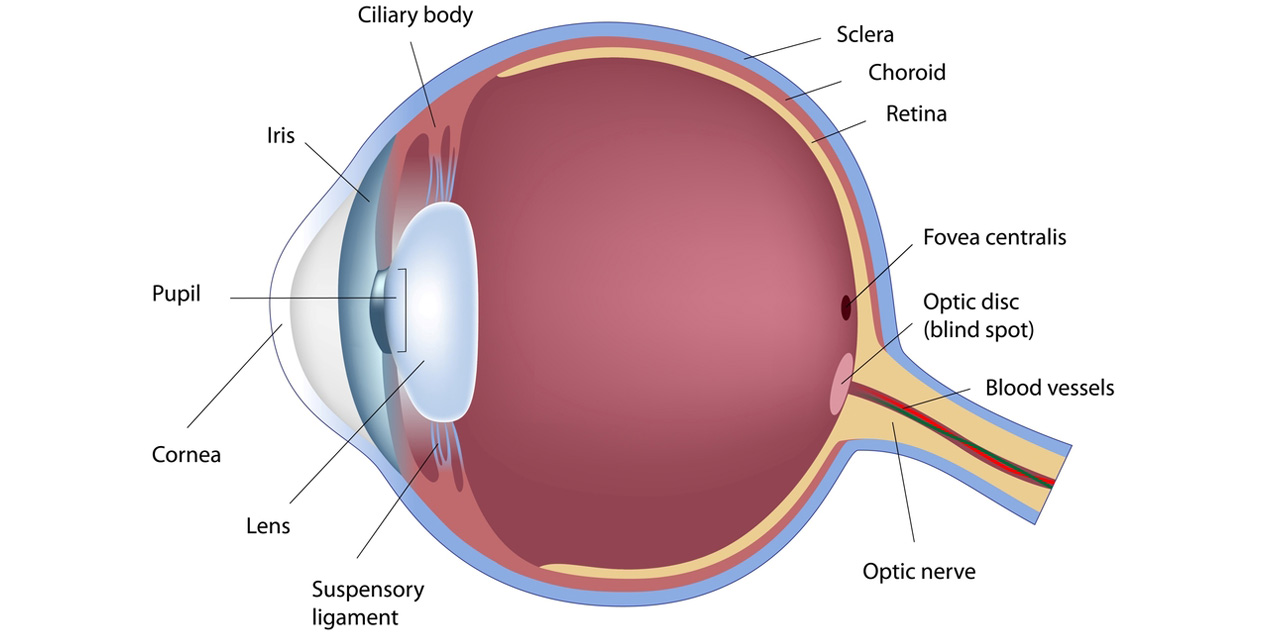
\includegraphics[width = 0.9\textwidth]{figures/Eye_anatomy.jpg} % scale, width, height 
  \caption{Anatomy of the Eye \cite{eyeimage}}
  \label{fig:Eyeanatomy}
\end{figure}  

Eye is one of the most important organs, which is responsible of vision for humans.
Saving this organ is critical and taking care of it is a must.
Many scientists have written the way the eye is working and they conclude, the eye is like a mirror so whatever it sees it reflects and in the very famous book (\textbf{Book of Optics}) \cite{alhazen1989book} written by Ibn Alhaytham, He claims "the eye is affected by light not the opposite".
In scientific view, the task of the eye is a sight machine that let the data received from the out atmosphere to be processed by brain for decision making for example: moving right ,left and etc... 
The camera idea was mainly gotten from the eye in the way it is working in term of light entrance to the lenses used then to the processor (Brain).
The camera creates pictures using films or digitally made \cite{abramoff2010retinal}.
Focus, contrast and the brightness also vary from camera to other based on how powerful the processor and other aspects.
The camera creates one image (Picture) or sequence of images (Video), it could be also in real time video like the eye with an advantage for the camera that it can record events for later use.
After observing how light travels by Ibn Alhaytham and his book he made the first pinhole camera to be the first design of camera and the development of the camera till our days.  
The anatomy of the eye is shown in Figure 2.1 with different layers, which is compromised with lenses to process data.
Humans may vary in the eye's structure, hence some people has a normal range of vision, others they can not see either far or near.
Eyes also can be infected by many diseases, which will be discussed after explaining the process of vision. 

Basically, the vision process can be explained as follows:
\begin{itemize}
\item \textbf{Cornea}: receives light for filtering.
Then, it focuses the data received.
\item \textbf{Aqueous Humour (Anterior Chamber)} : keeps the anterior part of the eye slightly curved and stable and it is made of viscous substance.
\item \textbf{Pupil}: adapts the eye lenses by relaxing or contracting depending on the amount of light enters the eye.
\item \textbf{Iris}: does the movement of the muscle based on the pupil order and based on the decision made by the pupil, the light will pass to retina
\item \textbf{Retina}: converts the light rays into electrical impulses to be delivered to the brain by optic nerve.

\end{itemize}
In our project we mainly focus in the retina part and it is explained as follows.

\subsubsection{Retina}
\begin{figure}[htb]
        \centering
        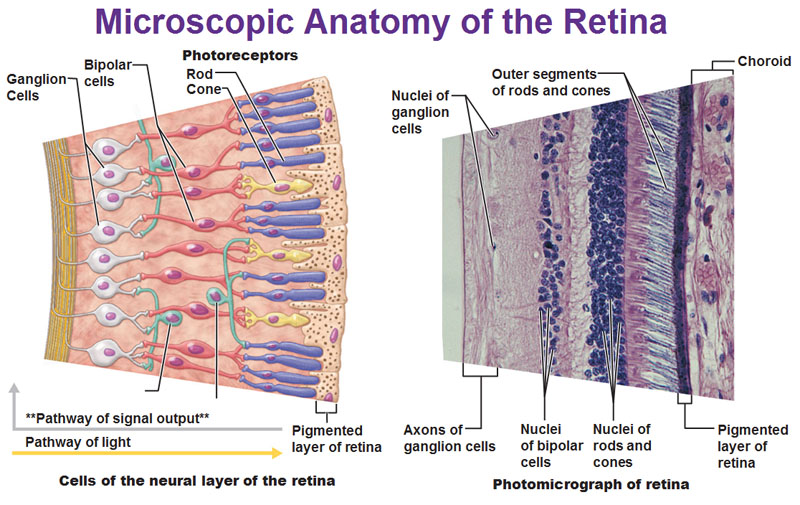
\includegraphics[width = 0.9\textwidth]{figures/Retina.jpg} % scale, width, height 
  \caption{Retina Anatomy \cite{retinaimage}}
  \label{fig:Retinaanatomy}
\end{figure}  
Retina is a multi-layered tissue located at the posterior of the eye.
Figure 2.2 shows the sensory parts in the retina, which they are the photo-receptors that get the rays and convert them into electrical impulses to be able to be read by the brain.
Impulses are passing through the optic nerve to the brain for image processing and the result of this process is the vision of the human.
There are millions of photo-receptors for sensing and there are two types of them based on their shapes : Rods and Cones.

Rods are located in periphery of the retina and they are imprecise and insensitive to colours so they can only recognize shapes in grey-scale.
Whenever there is a change in contrast it is very case-sensitive so it is most effective at night.
They are able to detect movement.    
Cones are responsible for day vision as they are very precise to detect colours.
They are located in the Macula \cite{mccaa1982eye}, \cite{abramoff2010retinal}.
The Fovea is the part of eye which is able to recognize the vision details. It is located in the central of the Macula.
Any accidental action to the eye results in losing Fovea will affect the vision in the central area.
A dense network of almost 1.2 million nerves is connecting the photo-receptors with the brain from the optic nerve.
The blind spot is located also in the retina, which has no photo-receptors.

The inner and outer layers of the retina  are encountered to be supplied by their fuel to enrich the retina with its need (oxygen and other important components required to keep the mechanism of vision) \cite{jonas1992count}.
The number of vessels for the inner layer 35\% is smaller compared to the outer layer 65\% to supply the retina.
Retina has many layers specified in \cite{abramoff2010retinal} as follows:
\begin{itemize}
\item Internal limiting membrane
\item Axons of the ganglion cells (Nerve Fibre Layer): the more the age, the thin it gets.
\item Ganglion Cell Layer includes the ganglion cells.
\item Inner Plexiform Layer have Amacrine and axons of bipolar cells.
\item Inner Nuclear Layer have horizontal and bipolar cells.
\item Outer Plexiform Layer includes horizontal dendrites and inner segments of photo-recepters cells.
\item The photo-receptors are located in the Outer Nuclear Layer.
\item External limiting membrane.
\item Finally, the layer that generates the colours to retina (Pigment Epithelium).
\end{itemize}
This complex combination of cells inside the retina is tremendous.
The existence of cysts is mysterious, thus it is studied by scholars to get the status of patients with different diseases \cite{jakobs2005retinal}

\subsection{Eyes Abnormalities}
Eyes abnormalities have no early signs, because the pain is not felt usually.
The vision also is not interrupted to give a warning that someone is infected by an eye disease to be diagnosed and get a treatment unless the problem is advance. 
As the body is a complex and compact system, hence any problem faces the eyes might interrupt many organs in the body and could be a sign to diagnose other diseases like heart diseases and diabetics.
The main disease, project making analysis on is the Diabetic Macular Edema (DME).

Diabetic sometimes called Diabetes mellitus (DM) where pancreas can not produce enough insulin or the cells can not respond to the insulin produced.
As of 2015, an estimated 415 million people have diabetes worldwide \cite{fernandez2010obesity}.
This represents 8.3\% of the adult population, with equal rates in both women and men \cite{vos2013years}.
The number of people with diabetes is expected to rise to 592 million by 2035 \cite{beagley2014global}.
The global economic cost of diabetes in 2014 was estimated to be \$612 billion USD \cite{atlas2013international}.
The best way to protect the eyes is by doing a regular visit to the doctor for eye examination.
Failing to treat this disease will yield to other diseases such as  cardiovascular disease, stroke, kidney failure and damage to the eyes.
In this section, many diseases that might hit the eye will be ordered alphabetically :
\begin{enumerate}
\item \textbf{Age-related Macular Degeneration (AMD)}: is a disease that will affect the Macula, which is located at the center of the retina.
Getting affected by AMD is a sign for diabetes.
AMD will lead to blur the vision, a dark area in the center of the vision and straight line distortion as shown in figure 2.3.
Activities required focus is affected by this disease like driving, cooking or studying.
There are two types of AMD: Dry and Wet. 
The wet AMD is happening due to generating new blood vessels in the Macula, which will lead to rapid lose of central vision.
In the other hand, dry AMD is happening due to the existance of drusen, which they are small yellow particles that they are deposited under the Macula.
Slowly, this particles will lead to lose the central vision and it is the most popular type \cite{bressler1988age}.
 
\begin{figure}[htb]
        \centering
        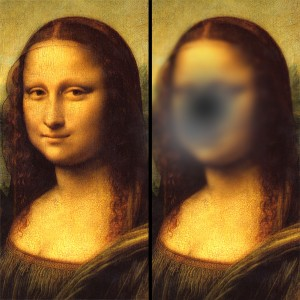
\includegraphics[width=0.45\textwidth]{figures/Centralloss.jpg} % scale, width, height 
  \caption{Loss of Central Vision \cite{centralloss}}
  \label{fig:Central Loss}
\end{figure}  
\item \textbf{Cataracts}: is an abnormality of the eye, which will affect the crystalline lens.
Crystalline lens is responsible in recognizing on stuff and people at different distances.
The typical effected patients in this syndrome is old people when the lens get stiffens due to ageing and they call it presbyopia.
In other ways, some people might face Cataracts earlier due to some reasons for example: diabetes, birth defects, steroids and heredity.
Cataracts patients will suffer from being sensitive to light, bad night vision, colour vision dimming, sometimes double vision in one eye and blurred vision \cite{klein1982cataracts}.
\begin{figure}[htb]
        \centering
        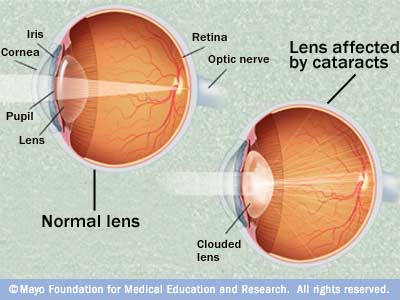
\includegraphics[width=0.7\textwidth]{figures/Cataracts.jpg} % scale, width, height 
  \caption{Cataracts \cite{cataracts2016}}
  \label{fig:Central Loss}
\end{figure} 
   
\item \textbf{Cytomegalovirus Retinis (CMV)}: is a disease that strikes the retina specifically the light sensing cells.
A quick treatment is required as this disease is so dangerous and sometimes might lead to blindness.
Cytomegalovirus Retinis does not produce symptoms and usually the immune system is able to fight it.
Sometimes, this virus will be accompanied by HIV virus.
This disease will make the patient suffer from couple of flashes for eyes, blind spots, end of the peripheral vision and blindness \cite{yeager1981prevention}.
\begin{figure}[htb]
        \centering
        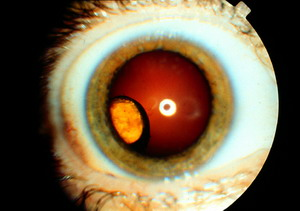
\includegraphics[width=0.3\textwidth]{figures/CMV.jpg} % scale, width, height 
  \caption{CMV and HIV \cite{CMV}}
  \label{fig:Central Loss}
\end{figure} 

\item \textbf{Diabetic Retinopathy (DR)} is disease that attacks the retina and it is a vascular complication.
Diabetic retinopathy (DR) is a vascular complication of DME that leads to vision loss in case of late treatment \cite{wilkinson2003proposed}.
Having Diabetes will increase the chances of getting blind than normal people.
\begin{figure}[htb]
        \centering
        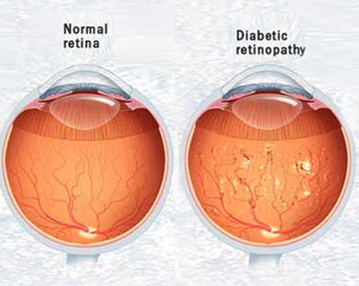
\includegraphics[width=0.6\textwidth]{figures/DR.jpg} % scale, width, height 
  \caption{Diabetic Retinopathy (DR) \cite{DR2016}}
  \label{fig:DR}
\end{figure}
\item \textbf{Diabetic Macular Edema (DME)} is a retinal disease and caused by fluid accumulation in the Macula dImaging of the eye is critical to improving the diagnosis, assessment of severity and progression, and evaluation of management of eye disease. 
It is also, a combination of complication of Diabetes Retinopathy that allows the fluid to escape.
The cones fill the Macula.
When the fluid starts to flow through the Macula to escape, blurred vision is the result of the inability of cones to sense the light.
Up to 30\% of Diabetes patients are suffering from DME. 
Two types of DME based on the way the fluid flow, which they are Focal DME and Diffuse DME.
To diagnose DME, retina thickness is checked if it is increased or exudate by 500 $um$ distance from the Macula centre \cite{bandello2010diabetic}.
DME only can be diagnosed by 3-D images because the lack of depth information when capturing the image due to the retina thickness increase.
Mainly, this project is focusing in detecting DME cysts and classifying the volumes based of how normal the volume is and DME shall look like the table in section 2.2.1

\item \textbf{Glaucoma}:this disease will damage the optic nerve, which is responsible for transferring data from the eye to the brain for image processing.
Thus, it will lead to vision loss or in the worst case scenario, blindness.
As other eye diseases, it is hard to diagnose the disease as it developed with no symptoms.
There are four types of Glaucoma: Chronic Open Angle Glaucoma, Acute Closed Angle Glaucoma, Secondary Glaucoma and Normal-Tension Glaucoma.
Glaucoma in case of acute angle will happen suddenly and the patient will vomit and feel dizzy. Also, it is accompanied with headache and vision blurring \cite{group1998comparison}.
\begin{figure}[htb]
        \centering
        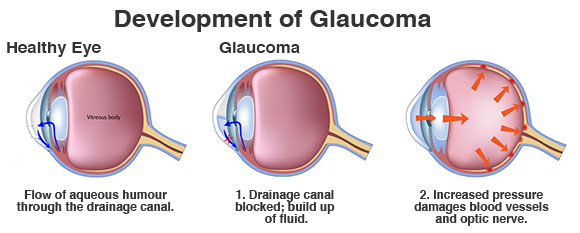
\includegraphics[width=0.75\textwidth]{figures/Glaucoma.jpg} % scale, width, height 
  \caption{Glaucoma \cite{Glaucoma}}
  \label{fig:Glaucoma}
\end{figure}

\item \textbf{Retinal Detachment}: a sudden damage of the retina allowing the fluid to flow inside it.
This action will make the retina to move away from the supportive tissue under it causing the detachment.
With this detachment, the retina is no longer able to correctly send the signals of light to the brain.
It can be treated but in a very good care \cite{retina1983classification}.
\begin{figure}[htb]
        \centering
        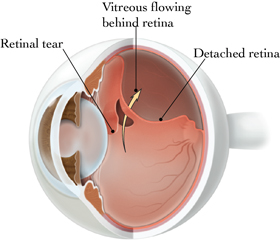
\includegraphics[width=0.5\textwidth]{figures/retinaldetachment.jpg} % scale, width, height 
  \caption{Retinal Detachment \cite{retinaldetachment}}
  \label{fig:Glaucoma}
\end{figure}
\end{enumerate}
 
\subsection{Imaging Techniques}
The eye imaging is critical in developing the diagnosing, analysing the progression and managing the evaluation of the disease.
The improvement in hardware such as chips and light sources and software such as image analysis is helpful in diagnosing the disease.
Based on the needed part of the eye and the disease to be imaged, the suitable imaging techniques are used by the ophthalmologists.
In this project, our data used are SERI and OPTIMA OCT images.
This section explains briefly ocular imaging techniques in the eye:

\begin{itemize}
\item \textbf{Scheimpflug principle}: this technique is named after its inventor the army captain Theodor Scheimpflug from Austria.
He has used it in creating a device for correcting the distortion in aerial photographs in a very systematic method.
This method has a rule that explains the orientation of the coordinates of optical system when the lenses are not in a parallel plane with the image plane.
It is can be used in corneal pachymetry, the corneal topography mapping, also prior to refractive eye surgery such as LASIK, and can be used in detection of keratoconus \cite{hockwin1987measuring}.
\begin{figure}[htb]
        \centering
        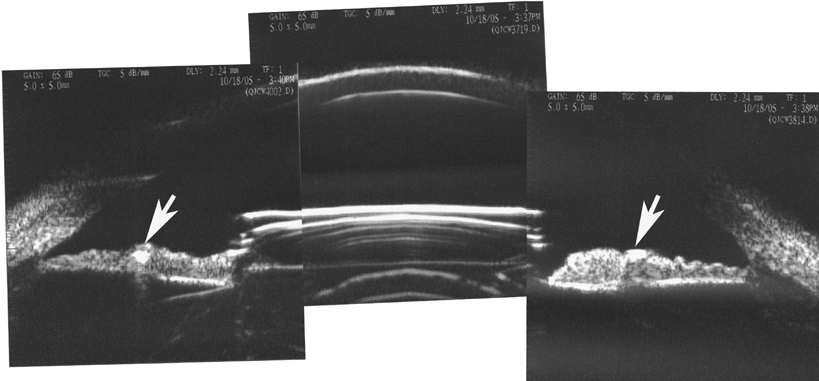
\includegraphics[width=0.7\textwidth]{figures/SPultra.jpg} % scale, width, height 
  \caption{Scheimpflug and ultrasonic \cite{SF2016}}
  \label{fig:Glaucoma}
\end{figure}

\item \textbf{Scanning laser ophthalmoscopy (SLO)}: this method is using confocal laser scanning microscopy for the aim of diagnosing the cornea and the retina at the eye of the human.
It employs scanning mirrors in horizontal and vertical coordinates for the aim of scanning a particular region in the retina and create a viewable images at the monitor.
It is also able to image the retina in real time and it might face a problem with reflections generated from the cornea.
It is helpful in term of diagnosing retinal disorders like DR, AMD, glaucoma and DME due to the high degree of spatial sensitivity \cite{gray2008vivo}.
It also has been developed to generate sharper images of the retina when it is combined with adaptive optics technology.
\begin{figure}[htb]
        \centering
        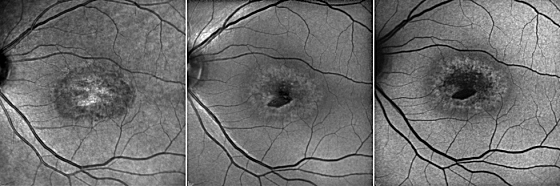
\includegraphics[width=0.6\textwidth]{figures/SLO.jpg} % scale, width, height 
  \caption{Scanning laser ophthalmoscopy \cite{SF2016}}
  \label{fig:Glaucoma}
\end{figure} 
\item \textbf{Ultrasonography}: this method uses mainly the time taken for high radio frequency pulses measurement, which is generated by piezoelectric devices.
The pulses is reflected by the interface of the ocular tissue(A-scan).
Another way of scanning (B-scan), which is inserting the probe across the eye to generate a section or moved in a rectangular pattern to create 3D form of structure \cite{cusumano1998three}.
As the emphasize of this method to use the high frequency pulses rather than light waves, it has the ability to penetrate opaque corneas to better image the ciliary body and surrounding parts.
Depth and resolution of ultrasonography penetration are affected by frequency's frequency.
\begin{figure}[htb]
        \centering
        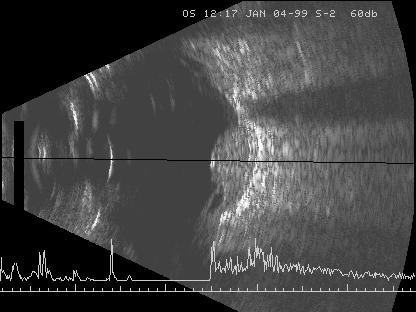
\includegraphics[width=0.4\textwidth]{figures/Ocularultra.jpg} % scale, width, height 
  \caption{Ocular Ultrasonography \cite{ocularultra}}
  \label{fig:Glaucoma}
\end{figure}
\item \textbf{Magnetic Resonance Imaging(MRI)}: is a well-known technique in imaging world, which results in producing a very detailed images of the internal frame of the body.
The principle of the MRI is based on nuclear magnetic resonance.
Spinning of the nuclei at certain radio frequency to obtain a stored signal that contains information about the the physical and chemical frame of molecules that has hydrogen.
Also, in the case of placing the object in an uniform magnetic field, the nuclear spins within the targeted structure.
Hence, they will align together wither in parallel or anti-parallel to the direction of the magnetic field flux.
Radio-frequency pluses will radiate echoes of the same frequencies which is detected.
The density of the nuclei and the internal structure will affect the magnitude and the decay of the signal.
Due to the high price of this device, so it has limited usage, but they use it in the ageing ciliary muscle diameter in phakic eyes \cite{strenk2004magnetic}, checking the 3D structure of the myopic, viewing gained ocular anomalies and some animal models in ocular drug-delivery systems\cite{kim2007assessment}.
\begin{figure}[htb]
        \centering
        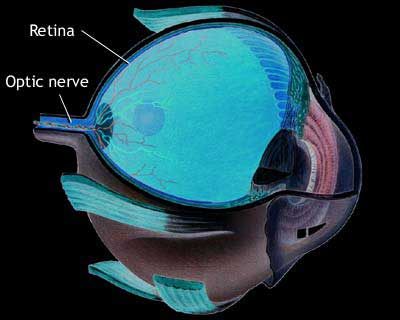
\includegraphics[width=0.3\textwidth]{figures/MRI.jpg} % scale, width, height 
  \caption{Magnetic Resonance Imaging \cite{MRI2016}}
  \label{fig:Glaucoma}
\end{figure}
\item \textbf{Optical Coherence Tomography (OCT)}: the main method of imaging in this project which is a light reflection based.
An interface is used instead of calculating the time between emission and detection of light-pulse owing to the fast speed of light in this technique, which is faster than sound speed in almost 872,000 times (344 $m/s$ speed of sound and OCT light speed is 299,792,458$m/s$).
Axial resolution is equal to light source coherence length and lateral resolution is the optics of the device function.
While, the laser (Conventional interferometry) has a long coherence length in meters, broadband of light sources are in use to make the laser frequencies shorten to micrometers in order to view high resolution eye image.
Any light outside the broadband of short frequencies length will not be used as data in the coherence pattern.
There are two types of OCT images, (A and B-scan).
A cross-sectional tomography (B-scan) is achieved by aligning a series of axial depths (A-scan).
(A-scan) is built by physically scanning the coherence length using the reference mirror in time domain OCT.
This type is limiting the resolution of the image and the images shall look like the table presented in section 2.2.1. 
(B-scan) is used to diagnose DME,AMD and Glaucoma with better precision than fundus images.    
\item \textbf{Optical Coherence Tomography Angiography (OCTA)} is another type of normal OCT, yet modern and from the name angiography, which means a technique to visualize the internal structure of organs and blood vessels.
OCTA uses motion contrast imaging to high-resolution volumetric blood flow data producing angiographic images in seconds.
OCTA matches the decorrelation signal (differences in the backscattered OCT signal intensity) between sequential OCT b-scans taken at accurately the same cross-section in order to create a map of blood flow.
Axial bulk motion from patient movement is removed so sites of motion between repeated OCT b-scans signify strictly erythrocyte movement in retinal blood vessels.
OCTA demands higher imaging speeds than most presently accessible OCT systems can deliver in order to attain a densely sampled volume.
Conventional OCT device scanning speeds would outcome in too much trade-off between reduced field of view, lower image quality, and greatly increased scanning time\cite{spaide2015retinal}.
\begin{figure}[htb]
        \centering
        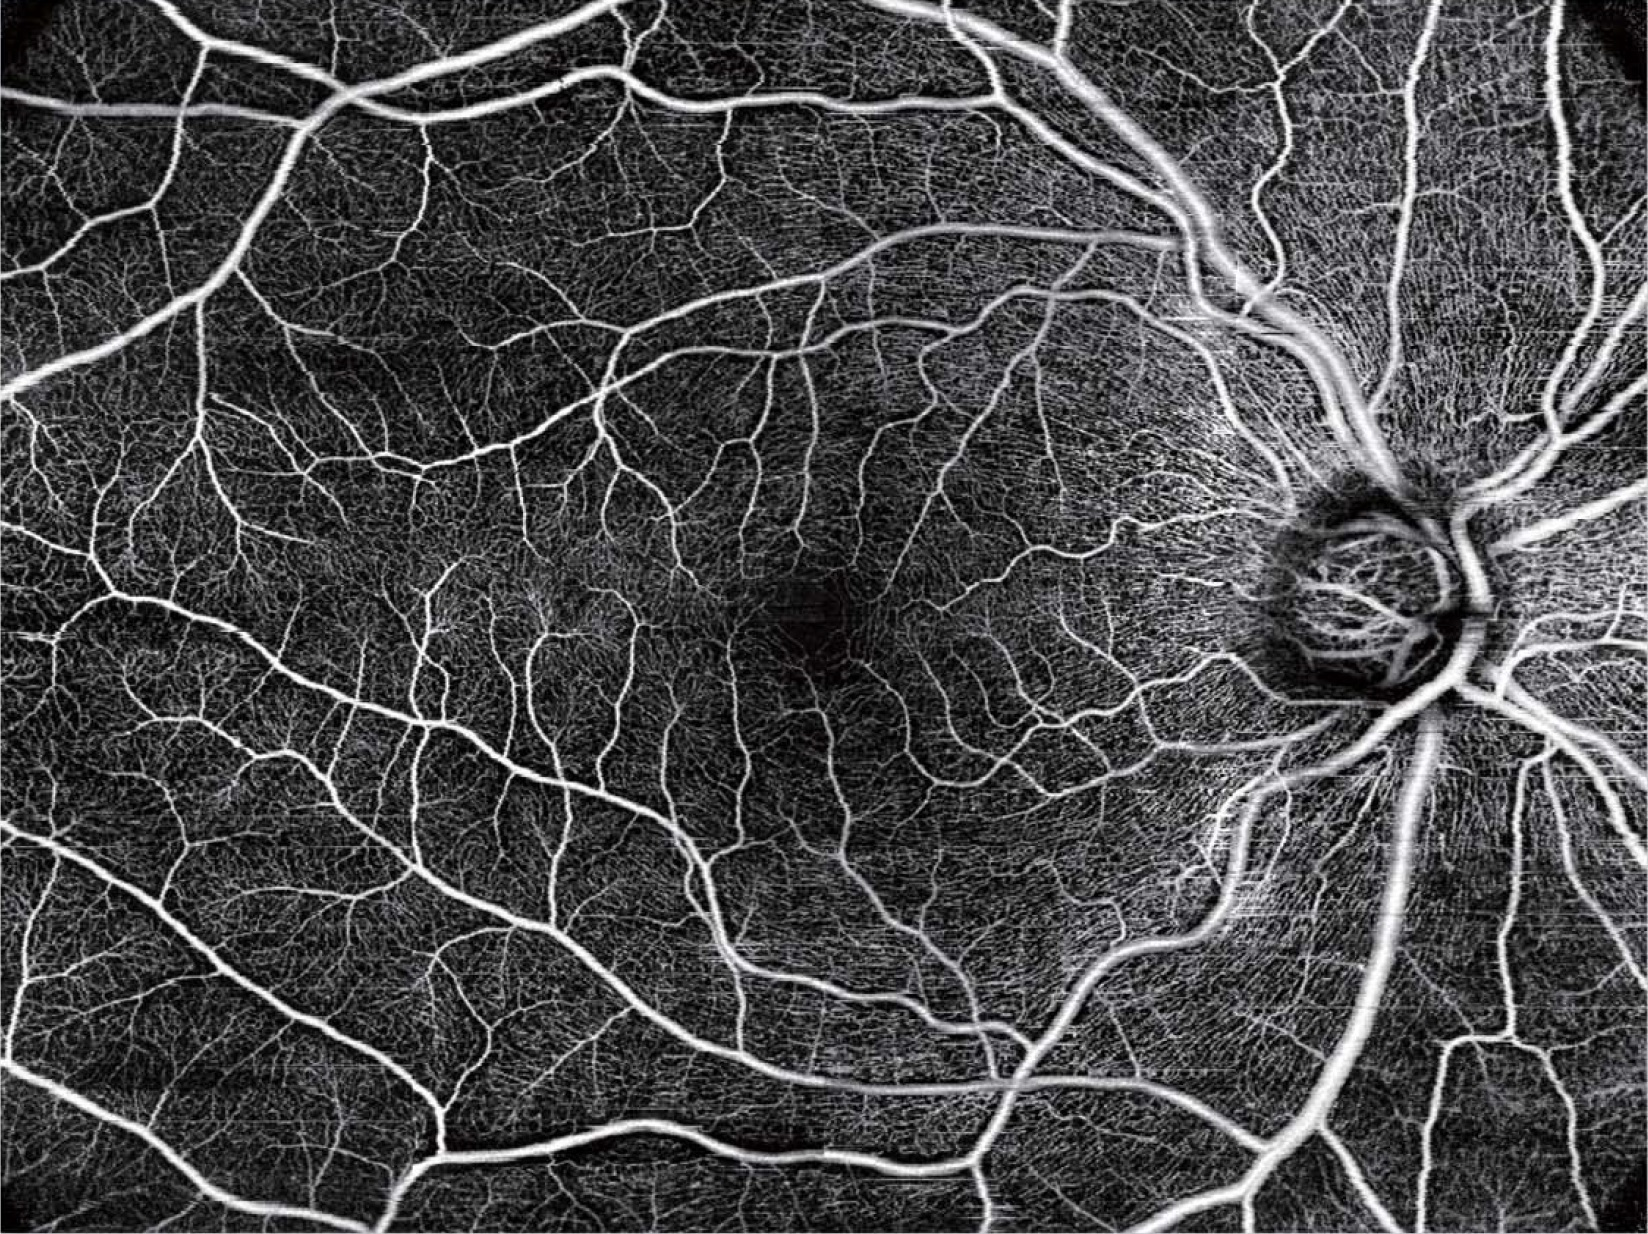
\includegraphics[width=0.3\textwidth]{figures/OCTA.jpg} % scale, width, height 
  \caption{Optical Coherence Tomography Angiography \cite{OCTA}}
  \label{fig:Glaucoma}
\end{figure}
\item \textbf{Fundus Photography}:is a method to screen the retina directly by using the pupil as the entrance and the exit of light rays for fundus camera.
The screening is achieved by placing the patient in front of the camera with the chin in a chin rest and the forehead against the bar.
Then, the photographer will align the camera and presses the shutter to fire a flash to create the fundus image\cite{sinthanayothin1999automated}.
Fundus images can be coloured with including some dyes like indocyanine and fluorescein.
\begin{figure}[htb]
        \centering
        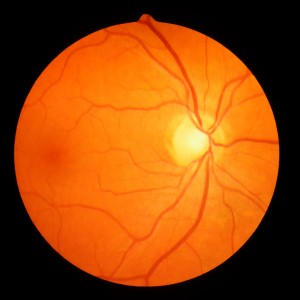
\includegraphics[width=0.3\textwidth]{figures/fundus.jpg} % scale, width, height 
  \caption{Fundus Photography \cite{fundus2016}}
  \label{fig:Glaucoma}
\end{figure}
\end{itemize} 

\section{Retina Analysis in OCT images}

In this section, previous work in the classification of the OCT images is presented and compared to have a better understanding of the field chosen.
Annotated data or dataset is required to diagnose the retina condition by analysing the retina morphology.
The design, implementation and testing of various previous work is reviewed.
There are many data for testing purposes and to be used with the permission of patients for scientific purposes.
Many datasets are available online for different parts or organs of the human body and also including the retina, where these datasets have different goals to study based on the case wanted to analyse.
The target in retina is different based on sickness needed to be diagnosed such as DME, AMD,DR, vessel segmentation and some localization tasks, hence many algorithms and datasets are done for each sickness to be diagnosed.
Since, the datasets are somehow useless if they are presented alone with no ground-truths aside the image or voxel to make the validation of the results and how accurate the designed algorithm.
By using the suitable method of image enhancing and extraction of data, ground-truth is giving a hand in training and testing data as the key to evaluate any algorithm's advantages and disadvantages.
This project used two types of data of OCT volumes, which they are SERI data and OPTIMA dataset.

\subsection{OCT Voxels Classification}
Over the past decades, the improvement in the applications of computer vision and image processing to
OCT volumes interpretation have been paid a big focus on improving an automated retinal layer
classification and segmentation methods.
This section discusses the recent state-of-the-art methods for classification using supervised and semi-supervised methods of SD-OCT volumes.
The datasets used in this study were acquired by the Singapore Eye Research Institute (SERI), using CIRRUS TM (Carl Zeiss Meditec, Inc., Dublin, CA) SD-OCT device \cite{cense2006ultra}.
The datasets consist of 32 OCT volumes (16 DME and 16 normal cases).
Each volume contains 128 B-scan with resolution of 512* 1024 pixels.
All SD-OCT volumes are read and assessed by trained graders and identified as normal or DME cases based on evaluation of retinal thickening, hard exudates, intraretinal cystoid space formation and subretinal fluid as presented in the table below.
Within the DME dataset, a large number of lesions were selected to create a rather complete DME dataset.
The volumes and sample numbers for DME volumes are presented in figure 2.4:
%\begin{figure}
%\centering
%        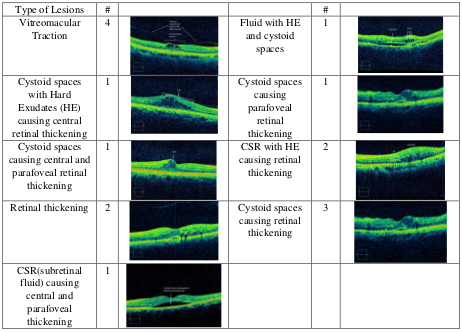
\includegraphics[width = 0.75\textwidth]{figures/bbdd.png} % scale, width, height 
%  \caption{Example of SERI dataset of DME}
%  \label{fig:SERI dataset}
%\end{figure} 

\begin{figure*}[t]
\begin{center}
   \subfigure[Vitreomacular traction.]{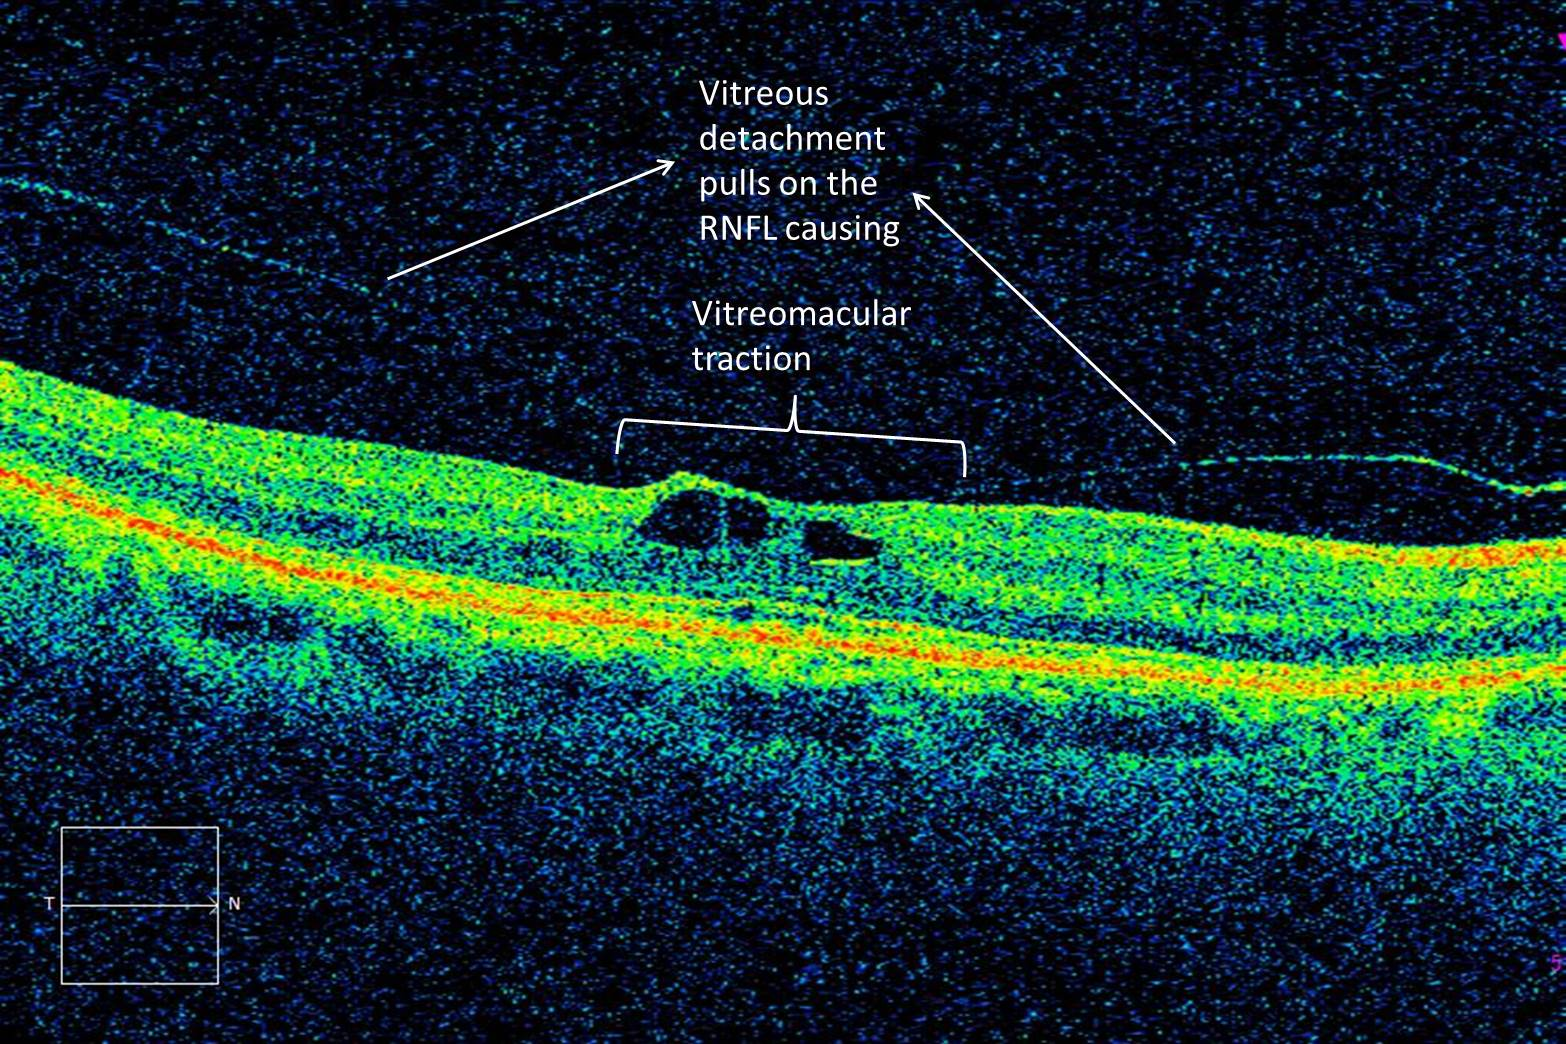
\includegraphics[width=0.3\textwidth, height = 0.15\textheight]{./figures/Vitreomacular}}\
   \subfigure[Rethinal thickening.]{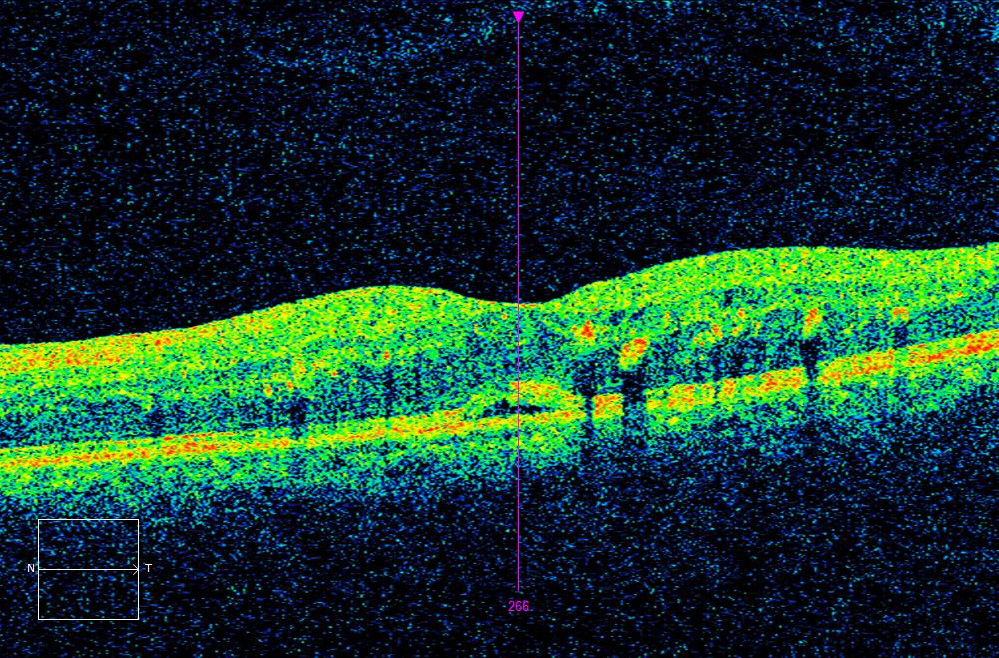
\includegraphics[width = 0.3\textwidth,height = 0.15\textheight]{./figures/RE}} \
   \subfigure[Cyst spaces, causing central and parafoveal retina thickening.]{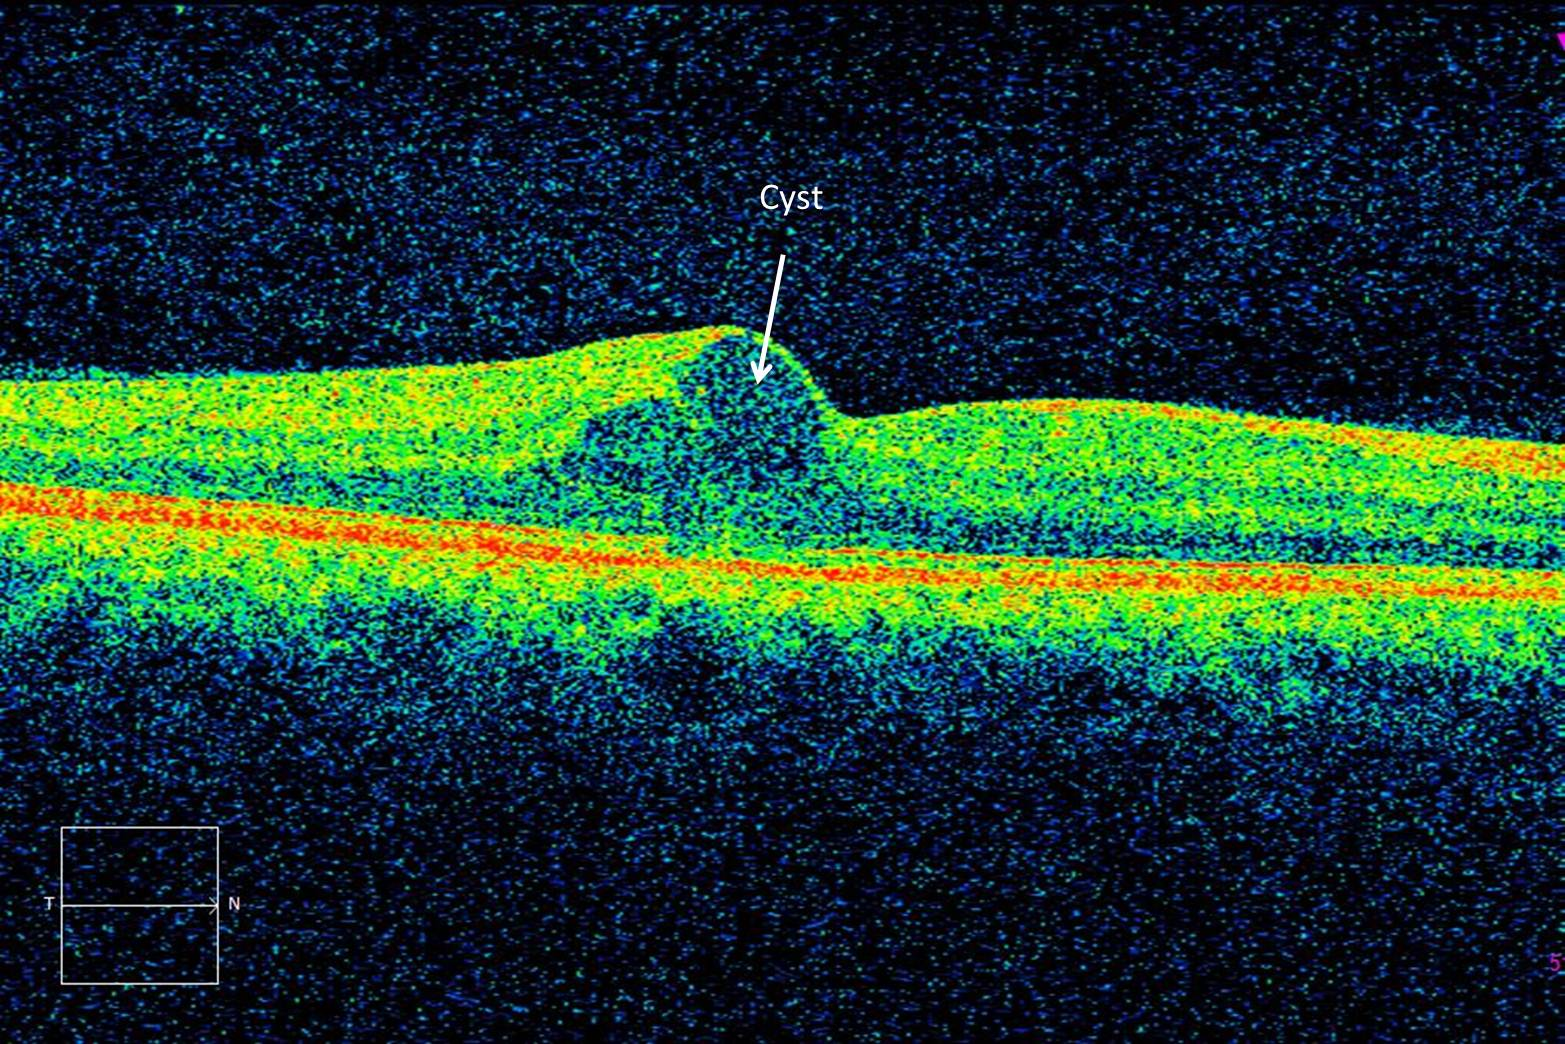
\includegraphics[width=0.3\textwidth,height = 0.15\textheight]{./figures/Cyst}}\\
   \subfigure[Cyst spaces and hard exudates, causing central retinal thickening.]{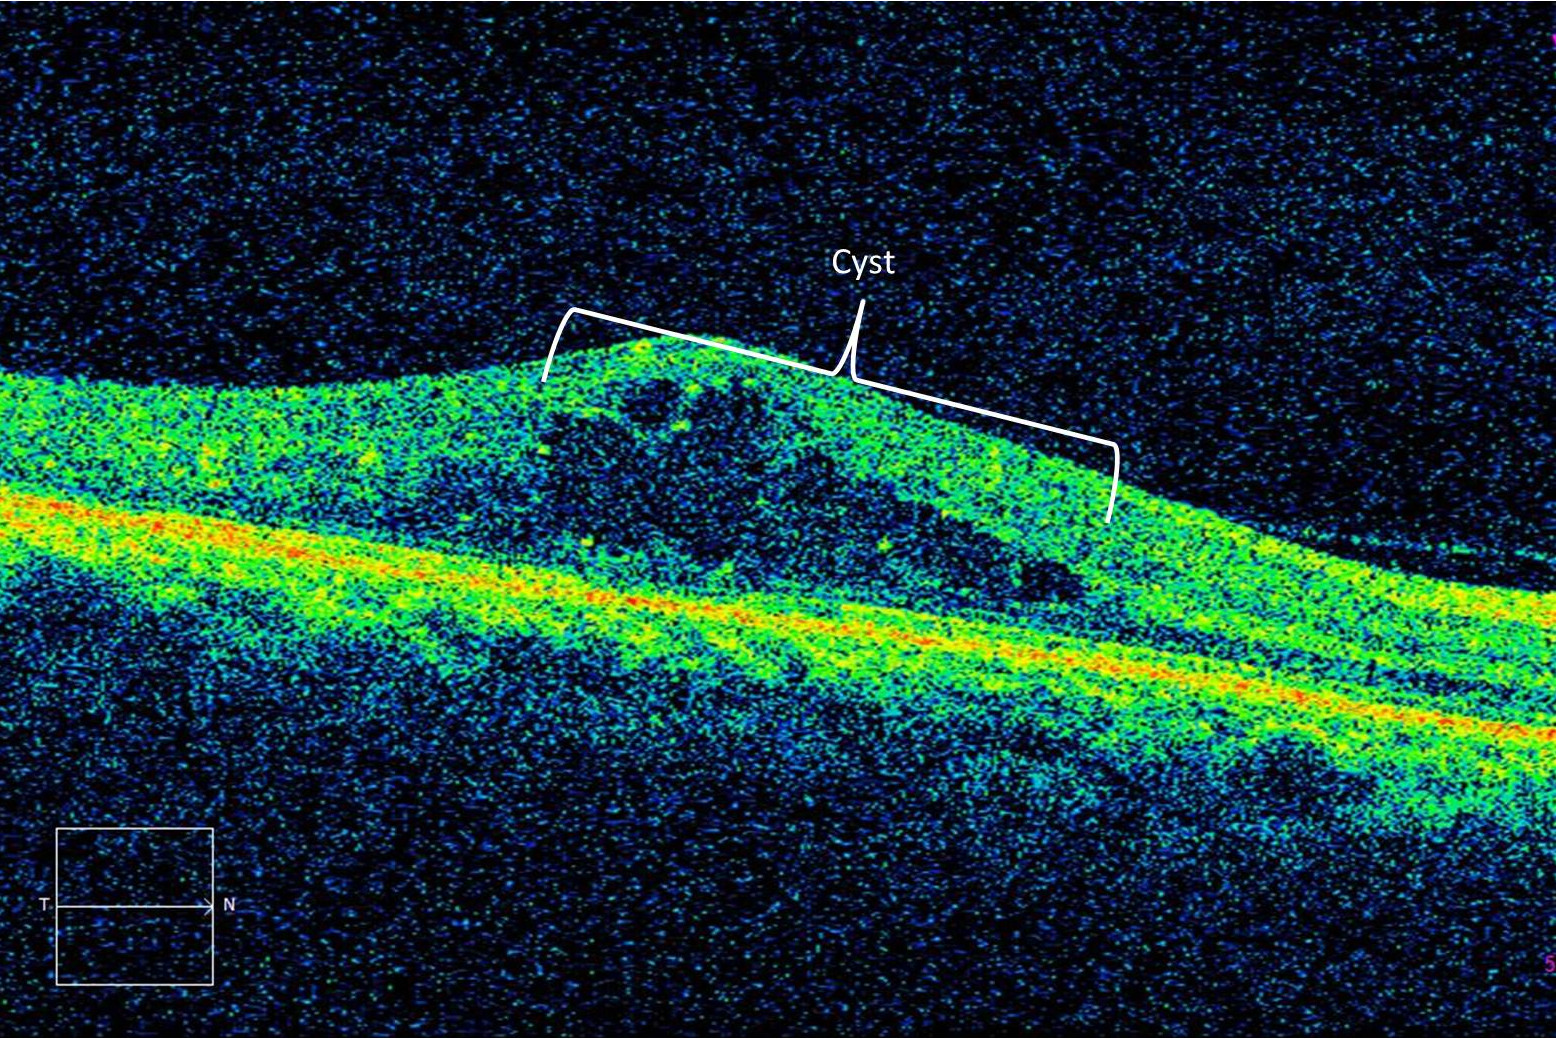
\includegraphics[width = 0.3\textwidth,height = 0.15\textheight]{./figures/Cyst+HE+RE}} \
   \subfigure[CSR (subretinal fluid), causing central and parafoveal thickening.]{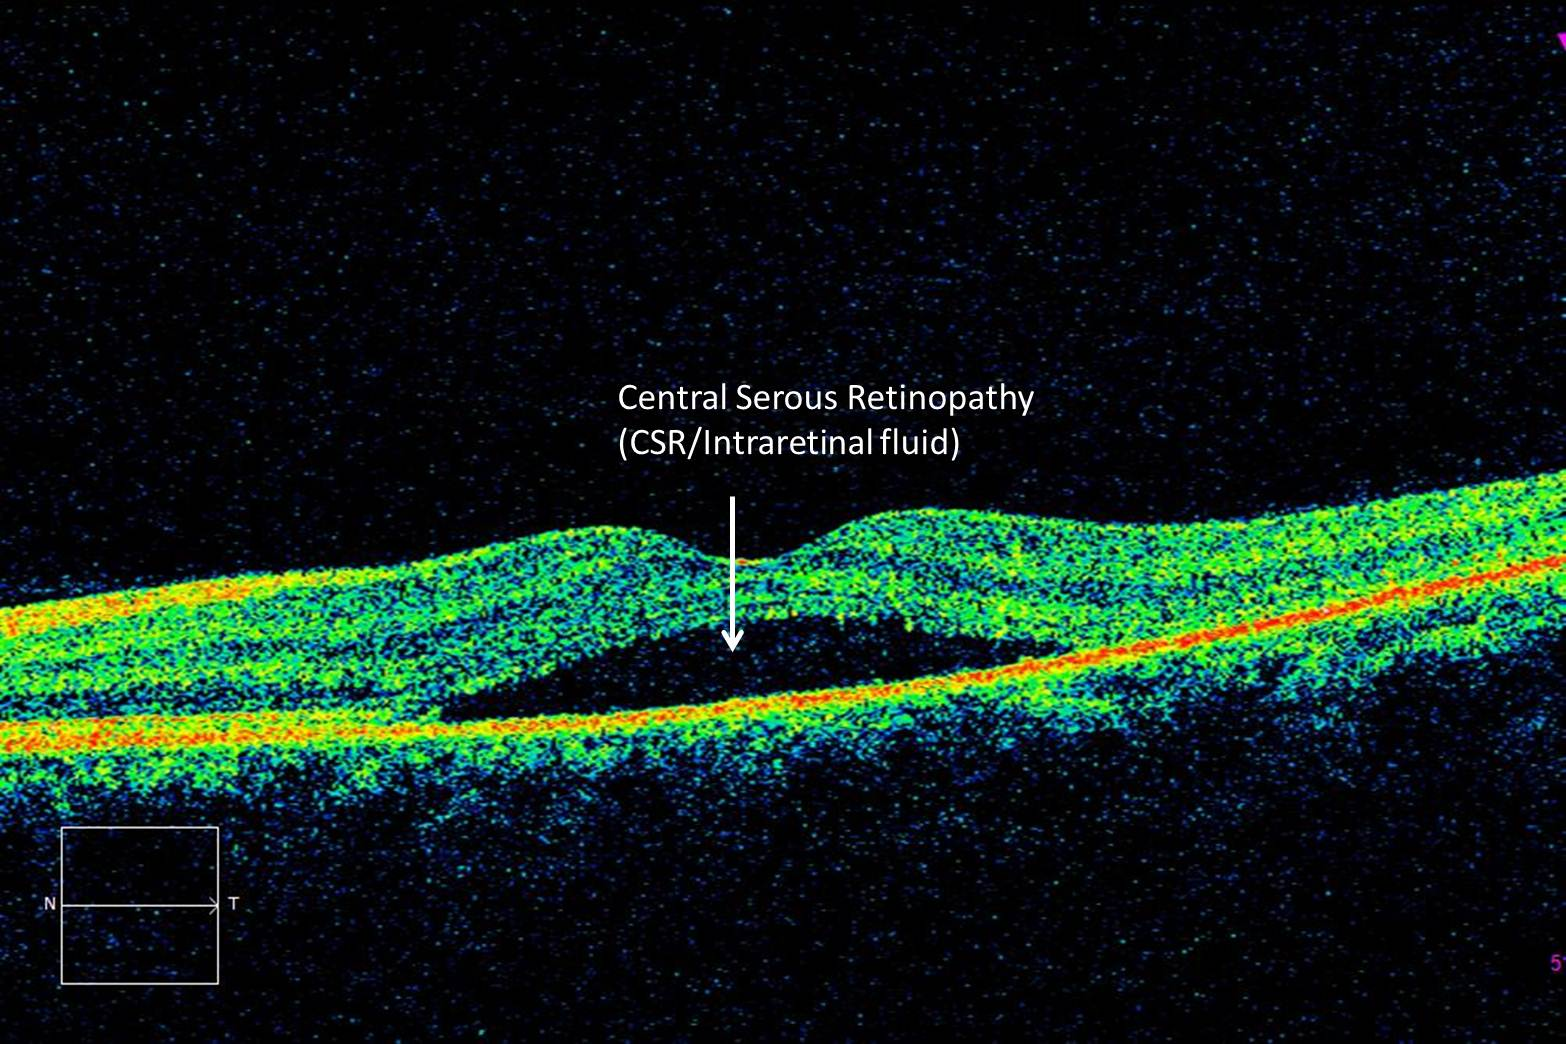
\includegraphics[width = 0.3\textwidth,height = 0.15\textheight]{./figures/CSR}} \
   \subfigure[CSR, hard exudates and cyst spaces.]{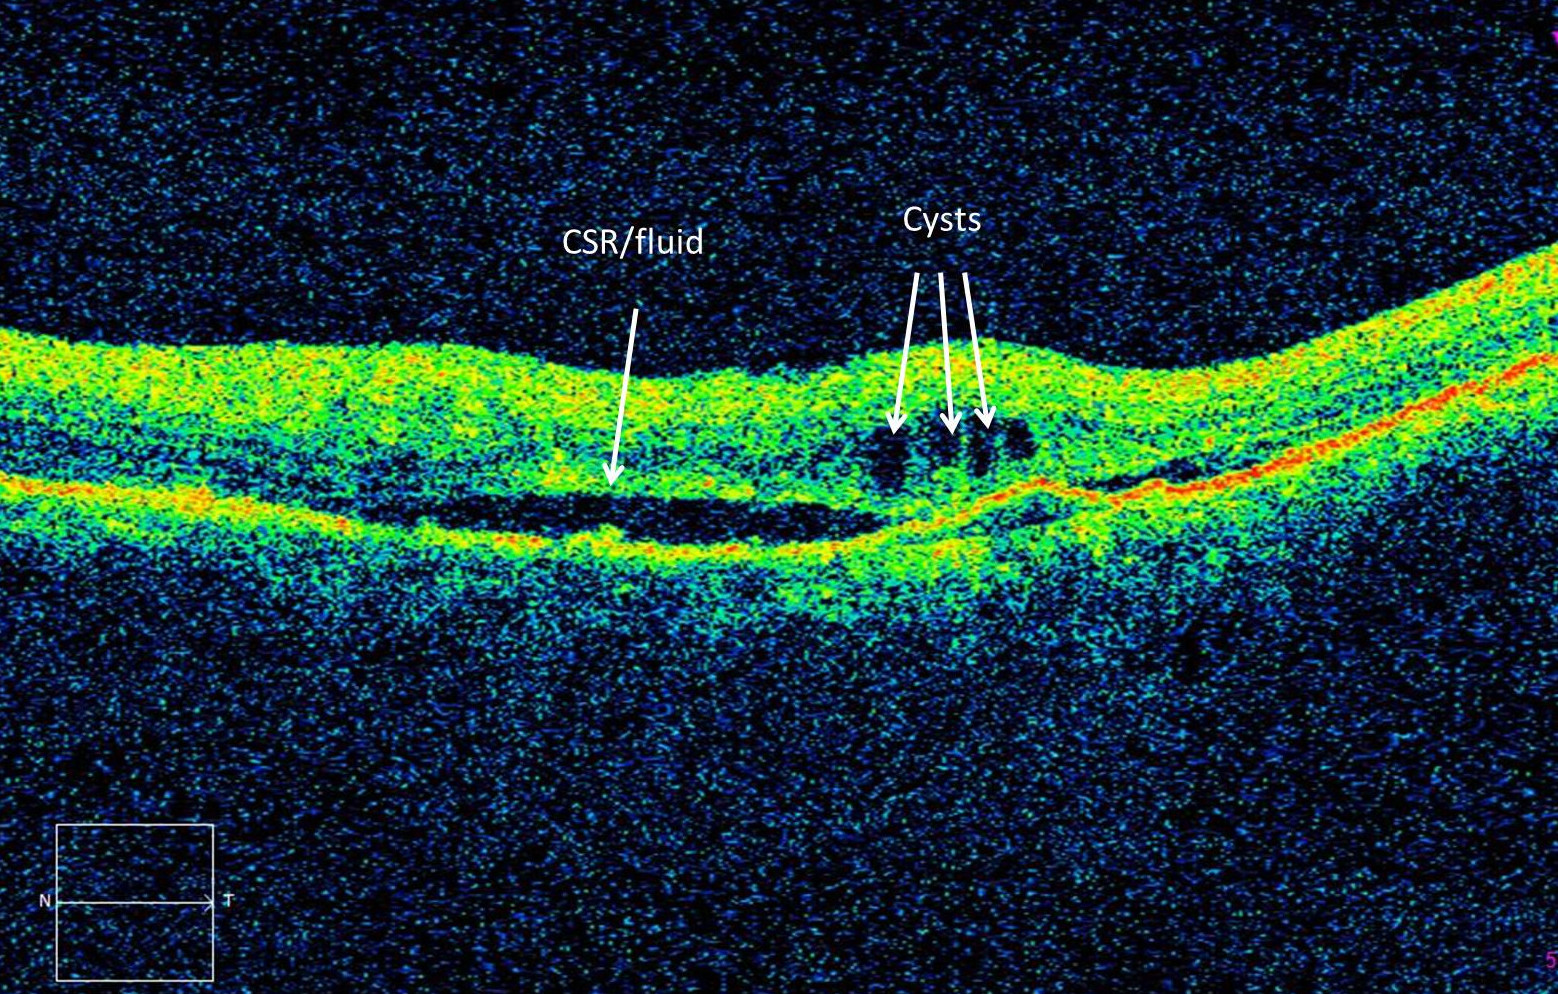
\includegraphics[width = 0.3\textwidth,height = 0.15\textheight]{./figures/Cyst+CSR+HE}} \\
   \subfigure[Cyst spaces, causing retinal thickening.]{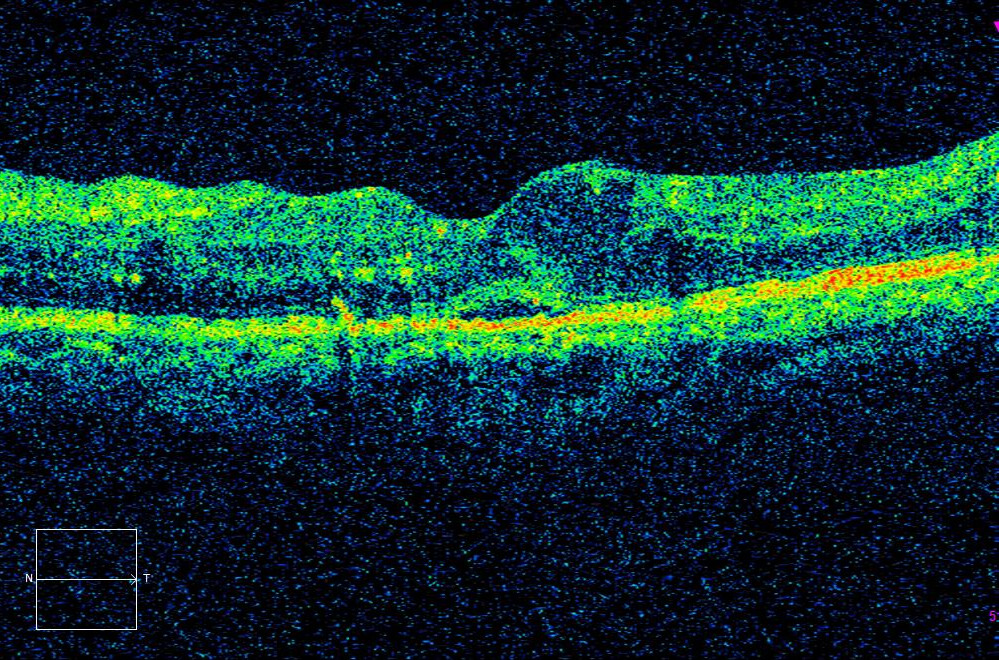
\includegraphics[width = 0.3\textwidth,height = 0.15\textheight]{./figures/Cyst+RE}} \
   \subfigure[CSR and hard exudates, causing retinal thickening.]{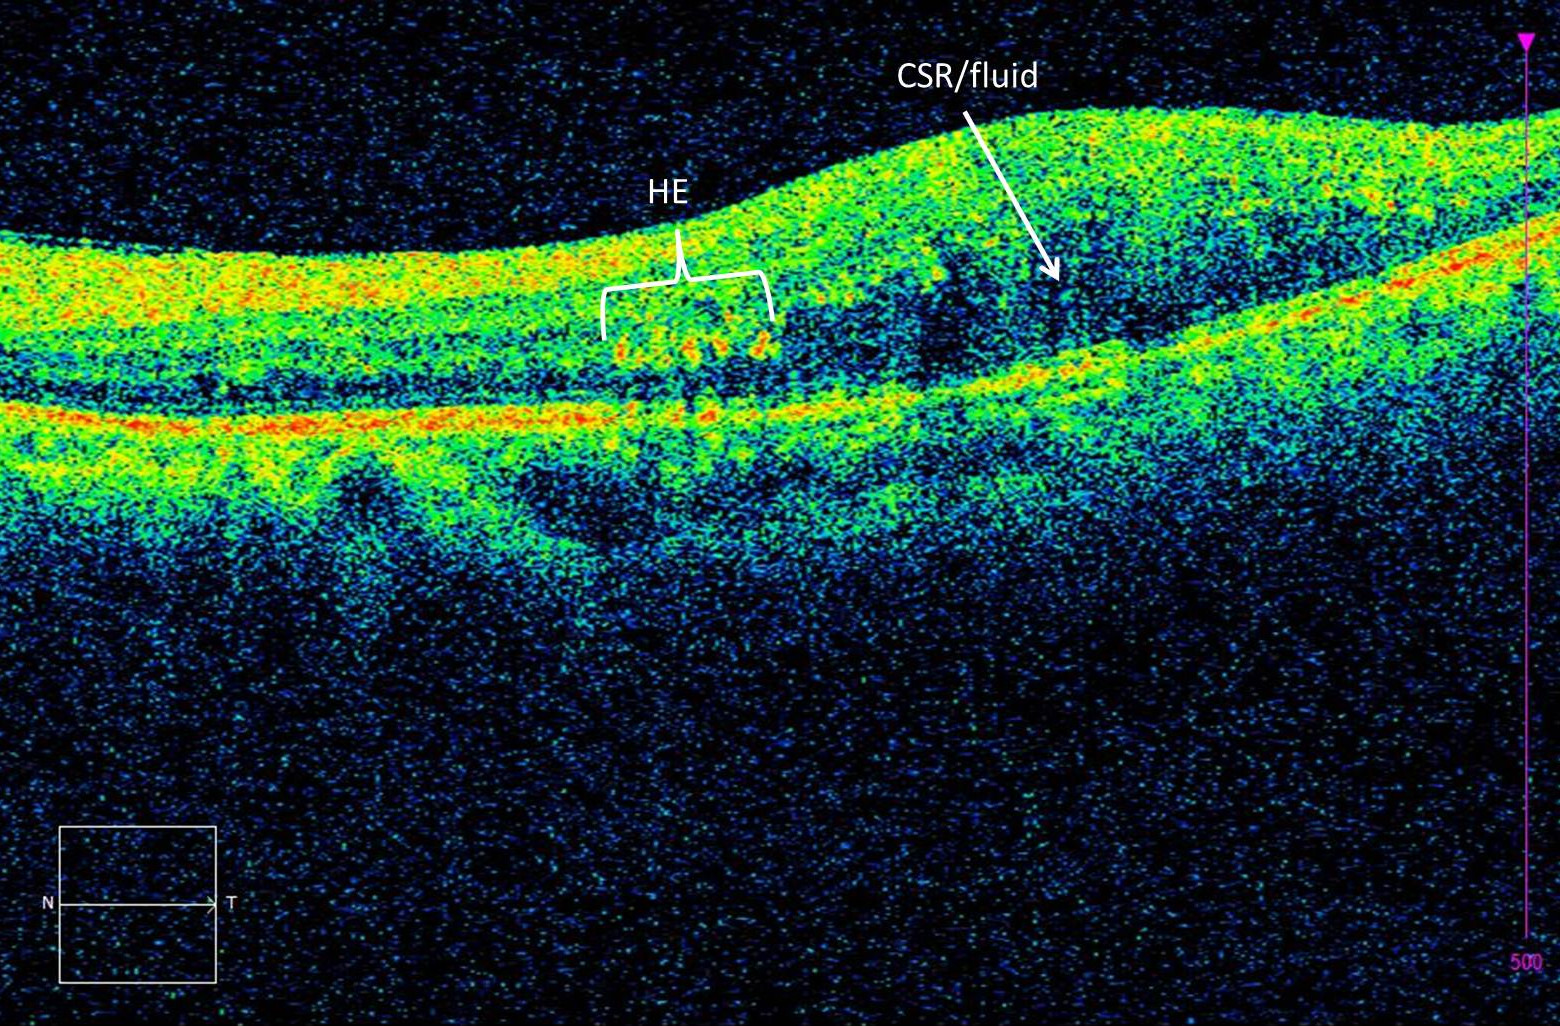
\includegraphics[width = 0.3\textwidth,height = 0.15\textheight]{./figures/CSR+HE+RE}} \   
   \subfigure[Cyst spaces causing parafoveal thickening.]{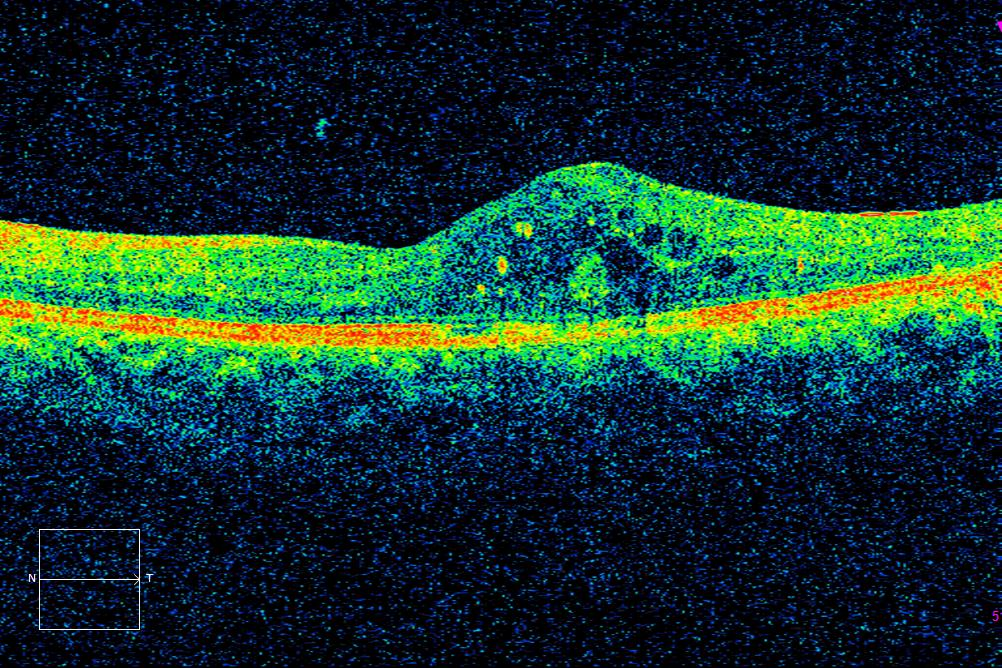
\includegraphics[width = 0.3\textwidth,height = 0.15\textheight]{./figures/Cyst+RE_parafovel}} \\
    
\end{center}
    \caption{Examples of \acs{dme} cases in \acs{seri} dataset.}
  \label{fig:bbdd}
\end{figure*}

Before, heading straight away to the algorithm, we shall know what is Machine learning.
Inventors have long dreamed and though of creating machines that are able to think just like humans.
The difficulties might face any systems depending on hard-coded knowledge said that Artificial Intelligence systems acquire the ability to have their own knowledge, by extracting features in patterns from raw data.
This capability is known as machine learning, essentially a form of applied statistics.
To have a precise definition we define what learning is first.
Learning is provided by \cite{mitchell1998introduction} \' A computer program is said to learn from experience E with respect to some class of tasks T and performance measure P, if its performance at tasks in T, as measured by P, improves with experience E\' .
And a human can imagine how computer can integrate couple of experiences, tasks and performances based on how powerful the computer is used for the particular task.
Tasks in machine learning can be classification, classification with missing inputs, regression, transcription, anomaly detection and many others. 

Srinivasan et al. propose a classification method to distinguish normal, DME, and Age-related Macular Degeneration (AMD) OCT volumes \cite{srinivasan2014fully}.
The SD-OCT volumes are enhanced by: 
\begin{itemize}
\item reducing the speckle noise through a de-noising method, which enforces the sparsity in a specific transform-domain.
\item flattening the retinal curvature.
\end{itemize}  
After that, edge information is extracted using Histogram of Oriented Gradients (HoG)descriptor for each B-scan of a volume and later used to train a linear Support Vector Machine (SVM).
This method is evaluated on a dataset of 45 patients equally subdivided into the three mentioned classes and led to a correct classification rate of 100\%, 100\% and 86.7\% for normal, DME and AMD
patients, respectively.
The dataset used by \cite{srinivasan2014fully} is publicly available but is already pre-processed (i.e., denoised, flattened, and cropped).
Furthermore, this dataset does not offer a huge variability in terms of DME lesions, have different sizes for the OCT volumes, and some of them, without specifying which, have been excluded during the training.
All these reasons, prevent us from using this dataset to benchmark our work.

Venhuizen et al. recently proposed a method to classify AMD and normal OCT volumes in \cite{venhuizen2015automated} using Bag of Words (BoW) models.
In the proposed method, the features are extracted from a set of key-points detected from each individual B-scan.
As a feature descriptor, a 9 px × 9 px texton is extracted around each selected key-point and its dimension is reduced, from 81 to 9 using Principal Component Analysis (PCA).
A dictionary or codebook is created by clustering the features extracted and each volume is represented in terms of a histogram, which captures the codebook occurrences.
These histograms are used as a final feature vectors to train a Random Forest (RF classifier.
This classifier is evaluated on a dataset composed of 384 volumes leading to an Area Under the Curve (AUC) of 0.984.

Liu et al. propose a methodology for detecting macular pathology in OCT images using Local Binary Pattern (LBP) and gradient information as attributes \cite{liu2011automated}.
Each B-scans is aligned and flattened and a 3-level multi-scale spatial pyramid is created. Additionally, edges are detected using Canny detector on the same pyramid.
Subsequently, an LBP histogram is extracted for each of the layer of the pyramid.
All the obtained histograms are concatenated into a global descriptor whose dimensions are reduced using PCA.
Finally, a SVM with an Radial Basis Function (RBF) kernel is used as classifier.
The method achieved good results in detection of OCT scan containing different pathology such as DME or AMD, with an AUC of 0.93 using a dataset of 326 OCT scans.

Lema\^{i}tre et al. propose another method based on extracted LBP features from OCT images and dictionary learning using BoW models \cite{lemaitre2015classification}. Contrary to \cite{srinivasan2014fully}, BoW and dictionary learning are used to perform volume classification is performed rather than B-scan. In this method, the OCT images are first pre-processed using Non-Local Means (NLM) filtering to reduce the speckle noise.
Then, the volumes are mapped into discrete set of structures namely: local, when these structures correspond to patches; or global, when they correspond to volume slices or the whole volume.
According to different mapping, LBP or Three Orthogonal Planes (LBP-TOP) texture features are extracted and represented per volume using histogram, PCA, or BoW.
The final feature descriptors per volumes are classified using RF classifier.
Classifying DME versus normal volumes on a balanced dataset of 32 SD-OCT volumes, the classification performance in terms of sensitivity (SE) and specificity (SP) of 87.50\% and 75\%, respectively, is achieved, while using LBP-TOP features and global mapping.

On the same dataset, Sankar et al. proposed a rather different approach, based on semi-supervised learning, to address the issue of an anomaly detection \cite{sankar2016classification}.
In their method, the authors proposed a technique that does not only allow the classification
of the OCT volume, but also enables the identification of the abnormal B-scans inside the volume.
This approach is based on modelling the appearance of normal OCT images with a Gaussian Mixture Models (GMM) and detecting abnormal OCT images as outliers.
The classification of an OCT volume is based on the number of detected outliers.
Testing on 32 OCT volumes, their proposed method achieved SE and SP of 93\% and 80\%, respectively.
A conclusion of this techniques is presented on table 2.1

\begin{table*}[t]
\caption{Summary of the state-of-the-art methods.}
\resizebox{1\linewidth}{!}{
\begin{tabular}{l ccc c cccc	c c c c	c c}
\toprule
References & \multicolumn{3}{c}{Diseases} & Data  & \multicolumn{4}{c}{Pre-processing} & Features & Representation & Classifier & Evaluation & Results\\
    &  &  &  & size &  &  &  &  &  &  &  & & &\\
   \cmidrule(l){2-4}\cmidrule(l){6-9} 
    & \acs*{amd} & \acs*{dme} & Normal  &           & De-noise & Flatten & Aligning & Cropping &   & &   &  &   \\
\midrule
& & & & & & & & & & & & & &  \\
Srinivansan~\textit{et~al.}~\cite{srinivasan2014fully} & $\checkmark$ & $\checkmark$ & $\checkmark$ &  45 & $\checkmark$ & $\checkmark$ &  & $\checkmark$ & \acs*{hog} &  & linear-\acs*{svm} & \acs{acc} & 86.7\%,100\%,100\%  \\
& & & & & & & & & & & & &    \\
Venhuizen~\textit{et~al.}~\cite{venhuizen2015automated} & $\checkmark$ &  & $\checkmark$ & 384 &  & & & &  Texton  &\acs*{bow}, \acs*{pca}  & \acs*{rf} & \acs*{auc} & 0.984 \\ 
& & & & & & & & & & & & &   & \\
Liu~\textit{et~al.}~\cite{liu2011automated} & $\checkmark$ & $\checkmark$ & $\checkmark$  & 326 &  & $\checkmark$ & $\checkmark$ &  &  Edge, & \acs*{pca}& \acs*{svm}-\acs*{rbf} &\acs*{auc} & 0.93 \\
& & & & & & & & &\acs*{lbp} & & & & \\
& & & & & & & & & & & & &  \\
Lema\^itre~\textit{et~al.}~\cite{lemaitre2015classification} &  & $\checkmark$ & $\checkmark$ & 32  & $\checkmark$ &  &  &  & \acs*{lbp}, & \acs*{pca}, \acs*{bow}&  \acs*{rf} & \acs*{se},\acs*{sp} & 87.5\%, 75\%  \\
& & & & & & & & &\acs*{lbptop} & Histogram & & &  \\
& & & & & & & & & & & & &  \\
Sankar~\textit{et~al.}~\cite{sankar2016classification} & & $\checkmark$ & $\checkmark$ & 32 & $\checkmark$ & $\checkmark$ & & $\checkmark$ & Pixel & \acs*{pca} & Mahalanobis & \acs*{se}, \acs*{sp} & 80\%, 93\% \\
& & & & & & & & &-intensities & &-distance to \acs*{gmm} & & \\ 
& & & & & & & & & & & & &  \\
\bottomrule
\end{tabular}}
\label{tab:survey-tab}
\end{table*}

\subsection{OCT Patch or Cyst Classification}
This section aims to explain the state of arts of work done in segmenting OCT voxels.
Inspired from the research done in segmenting OCT images, we did the classification on potential regions.
The SD-OCT data used in this project is provided by the OPTIMA laboratory (Christian Doppler Laboratory for Ophthalmic Image Analysis, Department of Ophthalmology, Medical University of Vienna) for the Cyst segmentation challenge hosted at MICCAI 2015.
These data consisted of 15 SD-OCT volumes containing a wide variety of retinal cysts with accompanying clinical ground truth annotation manually drawn by two different experts (Two Ground-Truths).
The SD-OCT voxels have 4 different vendors at different resolutions and scanning patterns: four volumes from Cirrus (Carl Zeiss Meditec, Dublin, CA, USA), three volumes from Nidek (NIDEK Co., Hiroishi, Gamagori, Japan), four volumes from Spectralis (Heidelberg Engineering, Heidelberg, Germany) and four volumes from Topcon (Topcon medical Systems,Santa Clara, CA, USA).
Results validation in this challenge were compared with the first and second reading by experts and the intersection between them compared to the segmented method done by the researcher.
Some examples of the Data used by Optima as shown in figure 2.16:
\begin{figure*}[t]
\begin{center}
   \subfigure[Cirrus-1.]{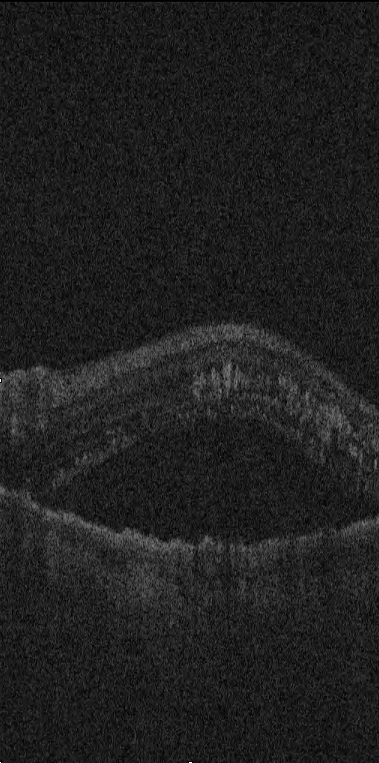
\includegraphics[width=0.4\textwidth, height = 0.2\textheight]{./figures/Cirrus_1.png}}\
   \subfigure[Nidek-1.]{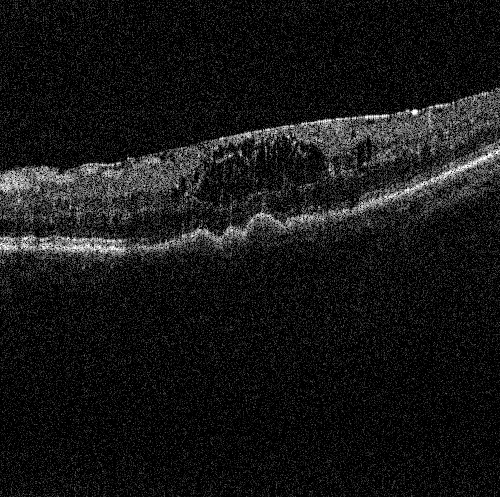
\includegraphics[width = 0.4\textwidth,height = 0.2\textheight]{./figures/Nidek_1.png}} \\
   \subfigure[Spectralis-1.]{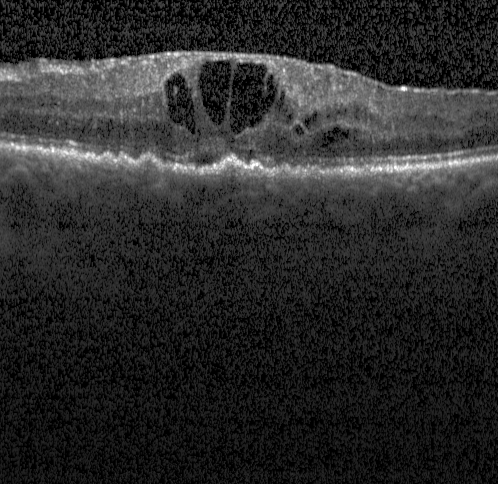
\includegraphics[width=0.4\textwidth,height = 0.2\textheight]{./figures/Spectralis_1.png}}\
   \subfigure[Topcon-1.]{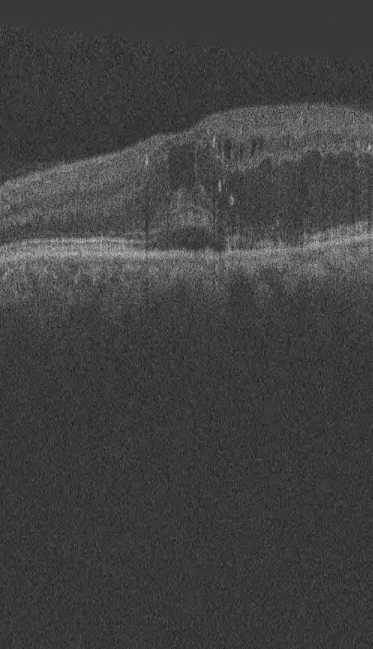
\includegraphics[width = 0.4\textwidth,height = 0.2\textheight]{./figures/Topcon_1.png}} 
   
\end{center}
    \caption{Examples of \acs{dme} and \acs{amd} cases in OPTIMA dataset.}
\end{figure*}

Many researchers went through this challenge made by Optima laboratory.
The method proposed by Luis et al \cite{LuisdeSisternes2015Optima} is a machine learning based, where a model is trained using manual markings (to establish the ground truth) and then tested using another 15 volumes of testing data also provided by OPTIMA laboratory.
In the preprocessing stage, the SD-OCT data normalized and de-noised using non-local means filtering in the axial and horizontal direction.
A defined number of boundaries defining the axial location of defined intra-retinal layers are then automatically outlined using a developed segmentation algorithm done by Luis et al in \cite{de2015localization} (SOARS: Stanford OCT Automated Retinal Segementation).
A number of quantitative features (34 features) are extracted to characterize each volume located between the segmented internal limiting membrane (ILM) and inner segment junction (IS), where the possible cysts are located in.
These features expanded to have four possible resolutions using multi-resolution approach to have set of predictors. 
After that, they calculate the risk score for each voxel.
The final segmentation output is generated automatically by detecting an adaptive threshold to
stratify the output scores in those belonging to a cyst or background.
The accuracy using this method has achieved a good results using dice coefficient evaluation with 80\% of correctly segmenting the B-scan slices.

Another proposed method by Ipek et al., \cite{oguz2016optimal}, which is using cost
function (opposed to machine-learned) that generalizes well to a variety of images.
This cost function takes into account the general characteristics of the input image as well as the well-known characteristics of fluid-associated abnormalities.
As the background and the cyst color in OCT images is black, so all methods care about certain area of the B-scan slice which lies between the layers.
They create a reliable mask even with the presence of fluid associated with cysts, followed by using a method to correct the Bruch membrane (BM). 
Then they segment using a cost function and they compare with the experts results.
This method fully cover all black holes lie in the layers and they did not target cysts only.

Mahdad et al., \cite{Mahdad2015Optima} used a speckle noise reduction algorithm, which maintains strong edge sharpness and reduce the noise.
This can be achieved by applying recursive Gaussian filter to noisy images and to any zero pixel exist in the image.
After that, threshold is used to the image to segment fluid space pixels.
Then nerve fibre layer (NFL) and retinal pigment epithelium (RPE) layer are extracted in each B-
scan.
Finally, most of the possible false positives (FPs) are removed based on standard deviation and morphology of extracted candidate pixels.

Another proposed method by Karthik in \cite{Karthik2015Optima} to segment OCT images.
They started by de-noising the image by using Total Variational approach that will reduce the texture content resulting in a smooth piecewise constant images preserving the edges.
Then, the make candidate selection as all methods done to specify the process only between NFL and RPE to save time and avoid pixels that they have nothing to do with the assessment of the disease existed in the voxel.
After that, Candidate regions are extracted using Maximally stable extremal regions(MSER).
This feature computation produces a set of stable region in an image.
MSER also used to detect the multi-scale objects without any smoothing.
Both small and large structure can be detected based on threshold and other aspects based on the favoured regions wanted to be extracted.
Then, based on the texture of pattern calculation, a local descriptor is assigned to each batch after making a bounding box for each region extracted by MSER.
Finally , with fifty trees in Random forest classifier is used for results validation and the results were challenging as it gives good results when the cyst is in medium and large size and poor results for small cysts.

A novel method using different way of training and extracting data proposed by Venhuizen \cite{venhuizen2015autCNN}.
His method mainly using the Convolution Neural Network to segment the images.
Two stages define the process, in the first stage, Three convolution neural networks (CNNs) are used to get a segmentation at different image scales.
In the second stage, the three CNNs scale segmentations are fused together, redefining the borders of the segmented cysts by combining local information obtained with the lower scale network with contextual information obtained from the higher scale networks.


%An image correspondence method is based on finding a mapping
%function ($f(x,y)$) that maps each coordinate of one image ($A$)
%into another image ($B$).

%\begin{equation}
%B(x',y')=A(f(x,y))
%\end{equation}
%\noindent  $B$.  $f_x$ and $f_y$(and $f_z$). 


%$m=(x',y')$ to its nearest point:
%
%\begin{equation}
%        B(m)=\sum_iw_i B(n_i)
%\end{equation}
%\noindent where each weight $w_i$ is related to the distance from
%$m$ (see Figure~\ref{fig:interp})
%
%\begin{equation}
%        w_1 = (1-dx)(1-dy) ~~~~ w_2 = (1-dx)dy ~~~~w_3 = dx(1-dy)
%        ~~~~ w_4 = dx dy
%        \nonumber
%\end{equation}


\appendix
\chapter{The first appendix}
If you need to add any appendix, do it here...
 Etc.

%   this is for BibTeX.  remove if you plan to write the references in the document
\bibliographystyle{plain}
\bibliography{refs}


%adds the bibliography to the table of contents
\addcontentsline{toc}{chapter}
         {\protect\numberline{Bibliography\hspace{-96pt}}}

\end{document}